\newpage
\section{Фоновые приложения в Windows}

\subsection{Службы Windows}

Служба (сервис от англ. service) - это программы, которые автоматически запускаются системой при загрузке Windows и выполняются в любом случае, вне зависимости от действий пользователя.

В большинстве случаев службам запрещено взаимодействие с консолью или рабочим столом пользователей (как локальных, так и удалённых), однако для некоторых сервисов возможно исключение — взаимодействие с консолью (сессией с номером 0, в которой зарегистрирован пользователь локально или при запуске службы mstsc с ключом /console).

Существует четыре режима для сервисов:
\begin{itemize}
\item запрещён к запуску;
\item ручной запуск (по запросу);
\item автоматический запуск при загрузке компьютера;
\item обязательный сервис (автоматический запуск и невозможность (для пользователя) остановить сервис).
\end{itemize}

Windows предлагает программу Service Control Manager, с её помощью можно управлять созданием, удалением, запуском и остановкой служб. Приложение, имеющее статус сервиса, должно быть написано таким образом, чтобы оно могло принимать сообщения от Service Control Manager. Затем, одним или несколькими вызовами API, имя службы и другие атрибуты, такие, как его описание, регистрируются в Service Control Manager.

Список служб находится в ветке реестра HKEY\_LOCAL\_MACHINE\textbackslash SYSTEM\textbackslash CurrentControlSet\textbackslash Services. Значения параметра «Start» имеют тип «REG\_DWORD» и могут принимать значения: «0», «1», «2», «3» и «4» (когда служба не запускается, то есть запуск данной службы запрещен)\cite{Cit5}.

Сервисы Windows по умолчанию запускаются от имени пользователя «LocalSystem», который обладает полными правами в системе (превосходящими права даже учётной записи Administrator). Рабочим каталогом будет системный каталог Windows (обычно C:\textbackslash WINNT или C:\textbackslash WINDOWS), а каталог для хранения временных файлов будет C:\textbackslash WINNT\textbackslash TEMP.

Поскольку это не настоящий пользователь, а «виртуальный», появляются некоторые трудности, когда приложению необходимо сохранить данные, относящиеся к пользователю (user-specific data), поскольку не существует папки этого пользователя.

Важно также то, что в случае если служба работает от имени локального пользователя (реальный пользователь созданный для служебных целей) если пароль такого пользователя изменён, сервис не будет запускаться до тех пор, пока пароль для сервиса тоже не будет изменен.

\subsection{Создание службы Windows с помощью программы Sc.exe}

Этот способ является рекомендованным корпорацией Microsoft\cite{Cit6}.

Для создания служб Windows можно использовать программу Sc.exe, включенную в пакет ресурсов Resource Kit, которая реализует вызовы ко всем функциям интерфейса прикладного программирования (API) управления службами Windows. Настроить параметры для этих функций можно, задав их в командной строке. С помощью средства Sc.exe имеется возможность запросить состояние службы и получить значения, хранящиеся в полях структуры состояний. SC позволяет задавать имя удаленного компьютера, что дает возможность вызвать функции интерфейса API службы и посмотреть структуры состояния службы на удаленном компьютере.

Кроме того, Sc.exe позволяет вызвать любую функцию интерфейса API управления службами и изменить любой параметр, используя командную строку. Данное средство предоставляет удобный способ создания и изменения записей службы в реестре и в базе данных диспетчера служб. Для настройки службы нет необходимости вручную создавать записи в реестре и затем перезагружать компьютер, чтобы обеспечить обновление базы данных диспетчером служб.

Программа Sc.exe использует следующий синтаксис:

\begin{Verbatim}[frame=single]
sc [Servername] Command Servicename
\end{Verbatim}

Команда \textbf{sc create} создает запись службы в реестре и в базе данных диспетчера служб.

Синтаксис
\begin{Verbatim}[frame=single]
sc [Servername] create Servicename [Optionname=Optionvalue...
\end{Verbatim}

Параметры могут быть следующими:
\begin{itemize}
\item Servername -- необязательный параметр. Задает имя удаленного сервера, на котором будут запускаться команды.
\item Command -- задает команду sc. Команды могут быть следующие:
\begin{itemize}
\item Config -- изменяет конфигурацию службы (постоянные параметры).
\item Continue -- посылает службе запрос Continue.
\item Control -- посылает службе запрос Control.
\item Create -- создает службу (добавляет ее в реестр).
\item Delete -- удаляет службу (из реестра).
\item EnumDepend -- перечисляет зависимости служб.
\item GetDisplayName -- указывает отображаемое имя службы.
\item GetKeyName -- указывает имя раздела службы.
\item Interrogate -- посылает службе запрос Interrogate.
\item Pause -- посылает службе запрос Pause.
\item qc -- запрашивает конфигурацию службы.
\item Query -- запрашивает состояние службы или указывает состояние по типам служб.
\item Start -- запускает службу.
\item Stop -- посылает службе запрос Stop.
\end{itemize}
\item Servicename -- указывает имя, присвоенное разделу службы в реестре.
\item Optionname -- служит для указания имен и значений дополнительных параметров.
\item Optionvalue -- задает значение параметра, которому присвоено имя параметром «Optionname».
\end{itemize}

Для выполнения ряда команд необходимо иметь права администратора. Следовательно, необходимо обладать правами администратора на компьютере, на котором создается служба.

Запустим netmonitor в качестве сервиса

\begin{Verbatim}[frame=single]
Sc create MyService binPath=C:\netmonitor.exe DisplayName=″My New Service″ type=own start=auto
\end{Verbatim}

По умолчанию создается служба типа WIN32\_SHARE\_PROCESS с типом запуска SERVICE\_DEMAND\_START. Она не имеет никаких зависимостей и выполняется в контексте безопасности LocalSystem.

Результат добавления приложения в список сервисов показан на рисунке 1.

\begin{figure}[H]
 \centering
 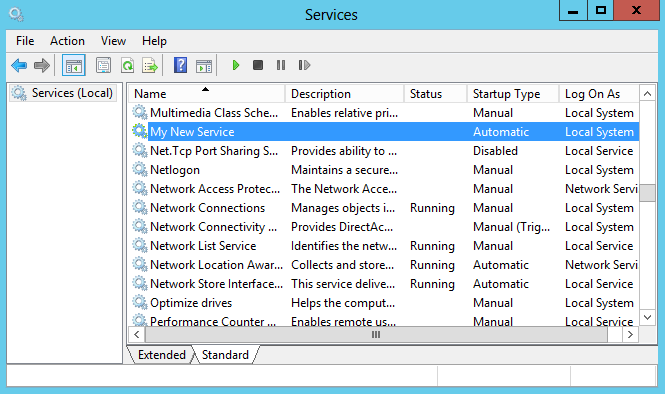
\includegraphics[scale=1]{res/pic001}
 \caption{Добавление сервиса из приложения в windows}
\end{figure}

\subsection{Создание службы Windows с помощью PowerShell}

Возможности управления системой из консоли в последних версиях Windows были значительно расширены. В том числе стало доступно и управление службами Windows. Создать новую службу можно с помощью командлета New-Service. Создадим такой же сервис, как и в предыдущем примере, только добавим к нему описание (Description):

\begin{Verbatim}[frame=single]
New-Service -Name MyService -BinaryPathName C:\netmonitor.exe`
-DisplayName ″My New Service″ -Description ″Very Important Service !!!″
\end{Verbatim}

Изменить параметры службы можно командлетом Set-Service:

\begin{Verbatim}[frame=single]
Set-Service -Name MyService -Description ″Not Very Important Service″ -StartupType Manual
\end{Verbatim}

PowerShell имеет примерно такой же функционал как и Sc.exe. Его особенностью является добавление описаний, но он не имеет простого способа удаления сервисов.

\subsection{Работа с системным журналом Windows}

Взаимодействие с системным журналом в Windows несколько сложнее, чем в Linux. Для начала требуется создать манифест (mc-файл) с описанием сообщений (листинг 2)\cite{Cit7}.

\lstinputlisting[language={},caption={mc-файл с описанием сообщений(src/daemons/win/eventlog.mc)}]{../../src/daemons/win/eventlog.mc}

Следующие две команды генерируют ресурсный файл и хедер для общения с этим ресурсным файлом.

\begin{Verbatim}[frame=single]
mc.exe -A -b -c -h . -r resources eventlog.mc
rc.exe -foresources/eventlog.res resources/eventlog.rc
\end{Verbatim}

После этого остаётся добавить eventlog.res при линковке бинарника, а eventlog.h подключить к основному модулю программы. Использование API системного лога Windows показано в листинге 3.

\lstinputlisting[language=C++, caption={Исходный код службы Windows, демонстрирующий API системного журнала (src/daemons/win/main.cpp)}]
{../../src/daemons/win/main.cpp}